% This is LLNCS.DEM the demonstration file of
% the LaTeX macro package from Springer-Verlag
% for Lecture Notes in Computer Science,
% version 2.4 for LaTeX2e as of 16. April 2010
%
\documentclass{llncs}
%
\usepackage{graphicx}
%\usepackage{makeidx}  % allows for indexgeneration
%
\begin{document}
%
\mainmatter              % start of the contributions
%
\title{Harnessing Wasted Computing Power for
Scientific Computing}
%
%
\author{S\'andor Guba \and M\'at\'e \H{O}ry \and Imre Szeber\'enyi}
%
\authorrunning{Ivar Ekeland et al.} % abbreviated author list (for running head)
%
%%%% list of authors for the TOC (use if author list has to be modified)
%\tocauthor{Ivar Ekeland, Roger Temam, Jeffrey Dean, David Grove,
%Craig Chambers, Kim B. Bruce, and Elisa Bertino}
%
\institute{Budapest University of Technology and Economics, Hungary,\\
\email{\{guba.sandor,orymate,szebi\}@iit.bme.hu}
}

\maketitle              % typeset the title of the contribution

\begin{abstract}
Nowadays more and more general purpose workstations installed in a student
laboratory have built in multi-core CPU and graphics card providing significant
computing power. In most cases the utilization of these resources is low, and
limited to lecture hours. The concept of utility computing plays an important
role in nowadays technological development. As part of utility computing, cloud
computing offers greater flexibility and responsiveness to ICT users at lower
cost.

In  this paper, we introduce a cloud management system which enables the
simultaneous use of both dedicated resources and opportunistic environment. All
the free workstations (powered or not) are automatically added to a resource
pool, and can be used like ordinary cloud resources. Researchers can launch
various virtualized software appliances. Our solution leverages the advantages
of HTCondor and OpenNebula systems.

Modern graphics processing units (GPUs) with many-core architectures have
emerged as general-purpose parallel computing platforms that can dramatically
accelerate  scientific applications used for various simulations. Our business
model harnesses computing power of GPUs as well, using the needed amount of
unused machines. This makes the infrastructure flexible and power efficient.

Our pilot infrastructure consist of a high performance cluster and 28
workstations with dual-core CPUs and dedicated graphics cards. Altogether we
can use 10,752 CUDA cores through the network.
% felére kell rövidíteni kb.

\keywords{Cloud, GPGPU, Grid, HTC, Utility computing}
\end{abstract}
%


\section{Introduction}
In universities there is a huge demand for high performance computing, but the smaller research groups can not afford buying a supercomputer or a large compute cluster. However significant unused computing capacity has been concentrated at fingertips in the student laboratories. Most of our student labs has quite new PCs with modern multi-core CPUs and high performance graphics cards. The total computing performance of the laboratory resources could be significant. The open questions are: a) how can we collect and use these resources; b) what is the time limit of the usage; c) what happens if one or more jobs are not finishing at the given time slot; d) what management software and management rules needed to support the various software environment which must be flexible and on demand. 

In this paper we are answering to these questions and we introduce a solution based on a new approach. We show that the cloud technology, based on hardware accelerated virtualization, can be the right answer to these question. First of all the management of the cloud based systems are easier and the they are more flexible. According to the literature [mate-kvm-performance] and our experience the modern virtualization has a minimal overhead to the native systems and has more advantages than disadvantages.

Our basic idea is to run only a minimal host operating system on the bare metal and virtualize everything else. In this manner we can easily solve the questions raised up. We do not need time consuming cloning process for the configuration management. We can save the ongoing scientific computing process at any time, and we can restore and continue it  even on other host machine.  One can say, yes, this goals are solved already by various cloud management systems in corporate environment. What is the novum on this? 

The main difference between the 7/24 hours cloud infrastructure and our laboratory environment is that the 7/24 hours infrastructure used only for serving the virtual machines.  The functions of student laboratory are twofold:  During the scheduled lab exercises the workstations act as a cloud host and/or  as a simple cloud client, which serves only the virtual machines owned by the student sitting in front of the workstation. 
However, the idle workstations acting as a normal cloud host running computing intensive jobs like a condor executing machine. 

 ----------------------------------------------------- itt tartok  -----------------------
One of the main differences between corporate and educational use is the count of users / count of workstations ratio, i. e. in student laboratories a single workstation is used by different persons each lesson.

Different hardware drivers, licensing and local storage limitations, or software incompatibilities all make system administrators maintain lots of different software environments. This process is both time-consuming and error-prone. Virtualization eliminates these combinations and provides the possibility of delegating special software installation to the lecturer. [n*m helyett n+m felet kell karbantartani] This introduces a way to rapid and frequent changes in the software environment.

\section{Virtualization}
Most IaaS (infrastructure as a service) cloud systems are based on virtual machines. Although the technique has been available since the end of 1960's, widespread adoption of x86 based systems in the server segment made it almost entirely disappear. Later some vendors started implementing different software based solutions for virtualizing operating systems or even emulating CPUs. The renaissance of virtualization began with manufacturers extending the x86 instruction set to  support low-overhead virtualization. This extension is known as Intel VT-x or AMD-V.

Current popular techniques are operating system virtualization and full hardware accelerated virtualization. The former typically takes shape in chroot environments and in namespacing of some kernel resources. This does not even allow running different kernels, nor different kinds of operating systems. The latest technique is full hardware accelerated virtualization, which is based on the CPU support for isolating the concurrently running instances. This approach is normally extended with paravirtualized device drivers, which eliminate the need for emulating real world storage and network controllers.

Hardware accelerated virtualization requires CPU support, but this is only missing currently on the low-end product line of the main x86 CPU manufacturers: some models of Intel Atom, Celeron, and Pentium. This hardware acceleration provides a near-native performance in HPC applications.[x]

Currently there are more competing full virtualization solutions, the most notable free ones are KVM and XEN. At the time of our decision, installing a XEN hypervisor required modifications to the Linux kernel, and this was unacceptable for us. This is no longer the case, but we are satisfied with KVM.

Also, we use all KVM functions through the libvirt library, which provides an abstract interface for managing virtual machines. This has the benefit of theoretically flawless migration to other hypervisors like XEN, ESXi, or Hyper-V.

Physically accessible computers are normally used with directly attached peripheries like display and keyboard. These devices are also emulated by KVM, and you can access virtual machines' consoles via the VNC protocol. This is useful for installing the operating system or troubleshooting, but Windows and Linux both provide better alternative for remote access.

We use remote desktop protocol for accessing Windows hosts, and secure shell for text-based Linux machines. Remote graphical login to X11 servers has always been available, but this is not reliable even on local network connections because it is stateless. We use instead NoMachine NX.


\section{Networking}

Most virtual machines in a cloud must have a network connection for obvious reasons.  When designing complex networks, the general approach is decomposition by (OSI) layers. That is what we will follow here.

On the physical layer, our KVM hypervisor gives us a virtual network interface controller, which is an emulated or paravirtualized NIC on the side of the guest operating system, and a virtual NIC on the host side.

Emulated network controllers are a good choice only for unsupported operating systems, as the solution is based on emulating a widespread real world network controller (i.e. the PCI signalling itself), and using a standard device driver in the guest operating system. This has a very significant overhead, limiting the available bandwidth to the 100Mbps order of magnitude even on the most powerful systems. On the other hand, virtio---the paravirtualized network interface of KVM---is able to transmit more Gbps without a significant CPU usage (our test measurements showed virtio 30 times faster than an emulated Realtek card).

Once we get a network connection between the host and the guest operating system, we have to connect the VM to the outworld. The most common solution to this is building a software based L2 (data link layer, Ethernet in this case) bridge of the virtual NICs and the uplink interface on the host machine. This is not a flexible solution, and provides poor management options like an unmanageable network switch does. Other option is using some trickery with ebtables, a not too widely known or documented Linux kernel service for ethernet filtering. It has some serious drawbacks, for example it can not use the same IP ranges on different virtual networks.

Manageable network switches are standard in operating dynamically changing and secure network infrastructure. Fortunately there exists an increasingly popular smart virtual switch implementation called Open vSwitch. It is a high performance multi-layer virtual switch with VLAN, QoS and OpenFlow support, merged into the mainline Linux kernel.

Our host systems are connected to manageable gigabit network switches' VLAN tagged ports. This renders it possible to connect virtual machines to isolated L2 networks on demand.

\begin{figure}[ht]
    \centering
    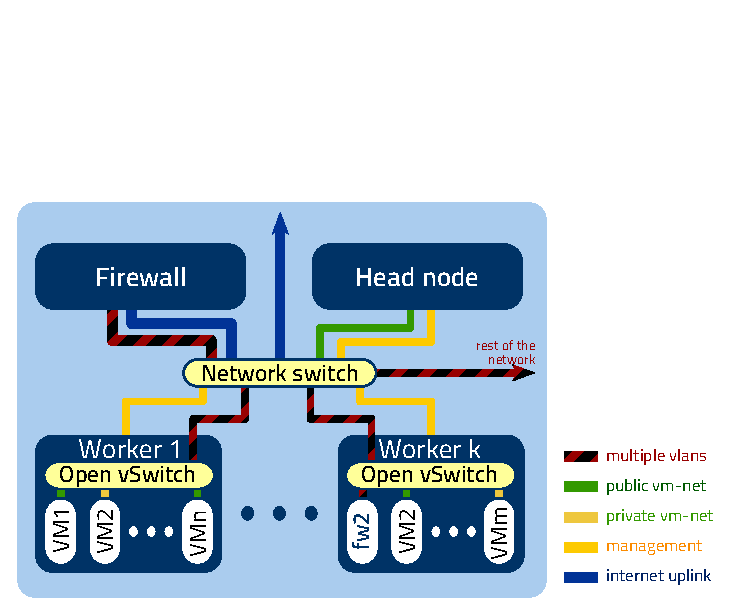
\includegraphics[width=10cm]{netarch}
    \caption{The physical structure of the network.}
\end{figure}

Open VSwitch is also configured to control network traffic according to the involved VM's QoS settings. Also basic protection is achieved using access control lists by prohibiting virtual machines egress traffic to use each other's allocated MAC or IP address.

Virtual networks are not very different from physical ones in the upper layers. The most important condition is the frequency of changes. Our system in traditional physical networks viewpoint is like if someone would change the cabling a hundred times in the middle of the day.

We have not found any friendly firewall and network gateway solution that supports this, or only a single one of our requirements: changing the network settings via remote procedure call, simultaneously changing the gateway, the name server and the DHCP servers' configuration, or supporting dynamically changing virtual networks (VLANs).

That is why we developed an integrated networking solution for all these requirements. Our system consists of an iptables gateway, a tinydns name server and an ISC DHCP server. All of these are configured through remote procedure calls, and managed by a relational database backed object model. This network management system also has a web interface, and can be used independently without a cloud. We also use the same system managing our physical infrastructure i.e. office and laboratory networks, traditional servers, and telephony.

We have a limited set of public IPv4 addresses, which is somewhat less than the number of currently running virtual machines. On the other hand, our IPv6 address space is more than enough for this.

Our solution is grouping the VMs to two main groups. The public vm-net is for machines which provide public services to more people, the private vm-net is for those which are used only by a single or a small group of persons.

Public vm-net machines have public IPv4 and IPv6 addresses, and are protected with a simple port based input filter (which is user-configurable). On the private vm-net, machines have private IPv4 and public IPv6 addresses. The primary remote connection is reached by automatically configured IPv4 port forward, or directly on the IPv6 address. As connecting to the standard port is a more comfortable solution, users who load our web portal from IPv6 connection, get a hostname with public AAAA and private A records. If the user has no IPv6 connection, we display a common hostname with a single A record, and a custom port number. As IPv6 is widely available in the central infrastructure of our university, IPv6-capable clients are in majority. Users can open more ports, which enable incoming connections, and set up IPv4 port forwarding.

As current implementations of DHCPv6 are not proper, we chose static configuration on the virtual machines. The allocated IP addressesanswer are specified in the contextualization configuration, and we anyway have to configure hostname, password, storage access, etc., so this was the simplest way. This method has also some performance advantage. We also configure DHCP, which is the preferred solution for non-virtualized workstations, or IP telephones.

\section{Storage}
For cloud system there is a need for a centralized storage system. It stores the virtual machine images accessible by all host machine. Basically there is two options for the 

The images stored on a central storage server and shared on NFS (Network File System). We store our images in QCOW (Qemu Copy on Write) format, which enables  separate base images and running instance differential images. This architecture enables fast virtual machine deploy without the need to copy full images on hosts.
	 	 	
CIRCLE Fileserver
Our first problem was that it is hard to exchange data with VM and if you delete the virtual machine all data will be lost. You can't connect USB drive and it is complicated to always install/use online storage solution in every VM you are using. We build a micro storage solution for our users. Virtual machines reach this server on local network via SSHFS or SMB protocol. The contextualized base images automatically connect these remote sources. Windows guest use SMB protocol and Linux/Unix guests use SSHFS. This is a persistent store and can be used on any VM. To manage the data outside virtual machines we build a webservice. It is bottle framework based RESTful API solution. After authentication our users reach their files like any other online storage solution. They can browse, download, upload, rename files and make or delete directories. You can mount your storage via sshfs at home. It's easy to to under Linux and Windows as well. The store is protected by key exchange authentcation. So to connect at home you need to upload your own publickey (openssh format) and you are ready to mount your remote filesystem.

Our cloud consist of two different part. The cluster responsible for running the critical services and virtual machines for students. Ant the lab computers for the opportunistic computing.


\section{Putting it together}
The main goal was to give a self-service interface to our researchers, lecturers, and students.
Cloud management frameworks like OpenNebula and OpenStack promise this, but after learning and deploying OpenNebula, we found even its Self-Service portal's abstraction level too low.

Our solution is a new cloud management system, code named CIRCLE (Cloud Infrastructure for Research and Computing Labs in Education). CIRCLE provides an attractive web interface where users can do themselves all the common tasks including launching and managing/controlling virtual machines, creating templates based on other ones, and sharing templates with groups of users.

\begin{figure}[ht]
    \centering
    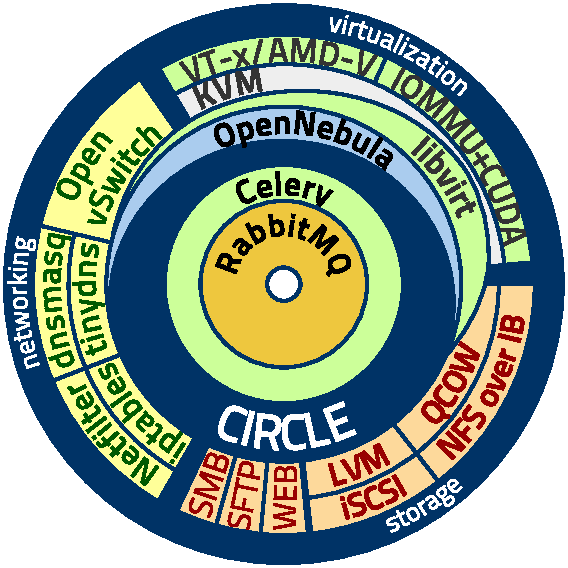
\includegraphics[width=8cm]{swarch}
    \caption{Technologies used for CIRCLE.}
\end{figure}

This cloud management system is based on Django. This popular Python framework gives us among other things a flexible object-relational mapping system. However the Django framework is originally designed for web applications, the business logic is not at all web specific. That's why it is easy to provide command line or remote procedure call interfaces to the model.

As the primary interface is web, which is in some aspect a soft real-time system, the model can not use synchronous calls to external resources, neither execute system commands. This is the reason why all remote procedure calls are done asynchronously through a standard task queue. Our choice is the most popular such system integrated with Django: Celery distributed task queue. Celery is configured to use an implementation of AMQP protocol---called RabbitMQ---as its message broker.

Celery workers set up the netfilter firewall, the domain name and DHCP services, the IP blacklist, execute file server operations, and also communicate with OpenNebula. This distributed solution makes it possible to dynamically alter the subsystems.

In the opposite direction, some subsystems notify others of their state transitions through Celery. Based on this information further Celery tasks are submitted, and the models are updated and persisted.

CIRCLE models manage the full state space of the resources. Some of it is also stored by the underlying OpenNebula, but most of this redundant information is bound to its initial value as OpenNebula does not handle changes in most of the meta information. This behavior arises of design decisions, and is not expected being improved.

The thin slice of OpenNebula used by our system is continuously shrinking, and we intend dropping OpenNebula in favor of direct bindings to libvirt and the also considerably customized storage and network hooks.

\section{Execution on workstations}
The cloud system at our institute takes a big role in education and in general R{\&}D infrastructure, but there is a significant demand for high-throughput scientific computing. This  kind of requirement usually appears in form of many long-running, independent jobs. On most parts of the world there is no fund to build dedicated HPC clusters with enough resources for these jobs.

The highest load on the cloud takes place in the public hours and the evenings, in more than half of the time we have much free resource, so it is accomplishable running these jobs on low priority virtual machines in the cloud. If interactive load is increasing, we can even suspend these machines, and resume them later.

Running scientific batch jobs on student laboratory computers also have a long history. Our idea is to run some of these jobs on virtual machines in the computer laboratories overnight and in the weekends. We can suspend in the morning all virtual machines to a memory image, and resume on the same or some other hypervisor next evening. This solution makes it possible to run individual jobs virtually continuously through months or a year, without any specific investment. This result is important because of our observation that the run length of similar jobs have a high standard deviation, and it also protects against losing the partial result of months long computations in case of hardware or power failure.

HTCondor has a similar result with its checkpoint support, but it needs modifying the software for this need, which is often impossible for proprietary products, or sometimes the user is not able to do this modification themself.

This solution uses mostly the same technologies as the dedicated cluster, but there are some different requirements originating from the distributed nature of a computer laboratory.

Computer laboratories have a 100Mbps Ethernet network, so using a read-write remote file system would damage the performance.

We can use a disk-cached read-only remote file system (NFS4 or CernVM-FS), and a local differential image (qcow2 or aufs). To be able to resume suspended machines, we have to copy back the differential image and the memory dump. Our choice for this is rsync.

This infrastructure can also be used without a notable modifications to run the short-term virtual machines of the student,who sits in front of the given workstation.

The lab network is exposed to unauthorized access, so we have to limit access to confidential material. As a physically accessible general purpose workstation does not currently have a way to reliably authenticate itself to a server, neither to protect the stored data, we can not employ any solution against these attacks other than security through obscurity and not using these systems for any confidential executions.

Other important aspect is energy efficiency. We have successfully used HTCondor to automatically turn on and off the compute nodes of a HPC cluster. This is also working with Wake on LAN and SSH on the workstations.

\section{GPUs in the cloud}
The most significant HPC performance in our student laboratories are the mid-level GPUs in all the workstations used for teaching computer graphics. There is a technology we used succesfully to use GPGPUs from the dedicated clusters' virtual machines: PCI passthrough. However this technology requires both CPU and motherboard support of IOMMU, which is a high-end feature nowadays. The implementations are called Intel VT-d and AMD-Vi technologies, and they appear in the server- and high-end workstation segments.

As none of our laboratory computers support IOMMU, we have to find a different solution. The first one is using rCUDA, which is a small framework making it possible to run host and device side of a CUDA program on different hosts, communicating over TCP/IP or InfiniBand network. With this, we can launch user-prepared virtual machines on each host, and run the device code via local (virtio-based) network on the hypervisor. rCUDA is also capable to serve more clients with a single device. This is useful if the host code uses the GPU only part time.

The other option is using directly the host machine to execute GPGPU jobs. This is a simpler approach, but necessarily involves a more complicated scheduler. Our choice for this type of problems is HTCondor, which can manage this scenario without much customization. The disadvantage is, that the user can't customize the host-side operating system.


\section*{Future}
Summary
ezen megy az oktatas a tavaszi felevben, statisztika, hany vm? user? 

The main cloud system described in sections 2 to 5 are fully functional. The extensions to support HTC on workstation however needs some more work at the time of writing this paper. Our plans are to make it fully functional, and release the whole system in an easily deployable and highly modular open source package. We are planning to finish the current development phase until end of August. 




%
% ---- Bibliography ----
%
\begin{thebibliography}{5}
%
\bibitem {clar:eke}
Clarke, F., Ekeland, I.:
Nonlinear oscillations and
boundary-value problems for Hamiltonian systems.
Arch. Rat. Mech. Anal. 78, 315--333 (1982)

\bibitem {clar:eke:2}
Clarke, F., Ekeland, I.:
Solutions p\'{e}riodiques, du
p\'{e}riode donn\'{e}e, des \'{e}quations hamiltoniennes.
Note CRAS Paris 287, 1013--1015 (1978)

\bibitem {mich:tar}
Michalek, R., Tarantello, G.:
Subharmonic solutions with prescribed minimal
period for nonautonomous Hamiltonian systems.
J. Diff. Eq. 72, 28--55 (1988)

\bibitem {tar}
Tarantello, G.:
Subharmonic solutions for Hamiltonian
systems via a $\bbbz_{p}$ pseudoindex theory.
Annali di Matematica Pura (to appear)

\bibitem {rab}
Rabinowitz, P.:
On subharmonic solutions of a Hamiltonian system.
Comm. Pure Appl. Math. 33, 609--633 (1980)

\end{thebibliography}

\end{document}
